\documentclass[a4paper, 11pt]{article}
\usepackage{comment} % enables the use of multi-line comments (\ifx \fi) 
\usepackage{lipsum} %This package just generates Lorem Ipsum filler text. 
\usepackage{fullpage} % changes the margin
\usepackage[a4paper, total={7in, 10in}]{geometry}
\usepackage[fleqn]{amsmath}
\usepackage{amssymb,amsthm}  % assumes amsmath package installed
\newtheorem{theorem}{Theorem}
\newtheorem{corollary}{Corollary}
\usepackage{graphicx}
\usepackage{tikz}
\usetikzlibrary{arrows}
\usepackage{verbatim}
\usepackage[numbered]{mcode}
\usepackage{float}
\usepackage{tikz}
    \usetikzlibrary{shapes,arrows}
    \usetikzlibrary{arrows,calc,positioning}

    \tikzset{
        block/.style = {draw, rectangle,
            minimum height=1cm,
            minimum width=1.5cm},
        input/.style = {coordinate,node distance=1cm},
        output/.style = {coordinate,node distance=4cm},
        arrow/.style={draw, -latex,node distance=2cm},
        pinstyle/.style = {pin edge={latex-, black,node distance=2cm}},
        sum/.style = {draw, circle, node distance=1cm},
    }
\usepackage{xcolor}
\usepackage{mdframed}
\usepackage[shortlabels]{enumitem}
\usepackage{indentfirst}
\usepackage{hyperref}
    
\renewcommand{\thesubsection}{\thesection.\alph{subsection}}

\newenvironment{problem}[2][Problem]
    { \begin{mdframed}[backgroundcolor=gray!20] \textbf{#1 #2} \\}
    {  \end{mdframed}}

% Define solution environment
\newenvironment{solution}
    {\textit{Solution:}}
    {}

\renewcommand{\qed}{\quad\qedsymbol}
%%%%%%%%%%%%%%%%%%%%%%%%%%%%%%%%%%%%%%%%%%%%%%%%%%%%%%%%%%%%%%%%%%%%%%%%%%%%%%%%%%%%%%%%%%%%%%%%%%%%%%%%%%%%%%%%%%%%%%%%%%%%%%%%%%%%%%%%
\begin{document}
%Header-Make sure you update this information!!!!
\noindent
%%%%%%%%%%%%%%%%%%%%%%%%%%%%%%%%%%%%%%%%%%%%%%%%%%%%%%%%%%%%%%%%%%%%%%%%%%%%%%%%%%%%%%%%%%%%%%%%%%%%%%%%%%%%%%%%%%%%%%%%%%%%%%%%%%%%%%%%
\large\textbf{\href{https://linkedin.com/in/Melvin-Mokhtari}{Melvin Mokhtari}} \hfill \textbf{Assignment 1} \\
Email: \href{mailto:melvin.mokhtari@ec.iut.ac.ir}{melvin.mokhtari@ec.iut.ac.ir} \hfill ID: 9831143 \\
\normalsize Course: Artificial Intelligence \hfill Semester: Winter 2023\\
Instructor: {\href{https://samanehoseini.iut.ac.ir/}{Dr. Samaneh Hosseini} \hfill Date: \today \\
%$22^{nd}$ November, 2019
\noindent\rule{7in}{2.8pt}
%%%%%%%%%%%%%%%%%%%%%%%%%%%%%%%%%%%%%%%%%%%%%%%%%%%%%%%%%%%%%%%%%%%%%%%%%%%%%%%%%%%%%%%%%%%%%%%%%%%%%%%%%%%%%%%%%%%%%%%%%%%%%%%%%%%%%%%%
% Problem 1
%%%%%%%%%%%%%%%%%%%%%%%%%%%%%%%%%%%%%%%%%%%%%%%%%%%%%%%%%%%%%%%%%%%%%%%%%%%%%%%%%%%%%%%%%%%%%%%%%%%%%%%%%%%%%%%%%%%%%%%%%%%%%%%%%%%%%%%%
\begin{problem}{1}
%Consider the scalar system
%\begin{align*}
%    \Dot{x} &= -x + u + w
%\end{align*}
%$w$ is zero-mean process noise with a variance of $Q$. The control has a mean value of $u_0$, an uncertainty of $2$ (one standard deviation), and is uncorrelated with $w$. Rewrite the system equations to obtain an equivalent system with a normalized control that is perfectly known. What is the variance of the new process noise term in the transformed system equation?
\end{problem}
%\begin{solution}
%The variance of the new process noise, $w_u$ is $\Sigma_{w_{u}} = Q + \sigma^2_u = Q + 4$.
%\begin{align*}
%    \Dot{x} &= -x + u_0 + \underbrace{w + \Delta u}_{w_{u}}, \quad w_u \sim (0, Q + \sigma^2_u).
%\end{align*}
%\end{solution}
\begin{solution}
\section*{\small Part 1}
Uninformed search, also known as blind search, is a search algorithm that operates without any prior knowledge or heuristics. It explores the search space systematically without any guidance or direction. On the other hand, informed search, also known as heuristic search, uses some prior knowledge, domain-specific heuristics, or other intelligent strategies to guide the search process towards the goal.\\
Here are some advantages of uninformed search:
\begin{enumerate}
\item Simplicity: Uninformed search algorithms are usually simple and easy to implement.
\item Completeness: They are guaranteed to find a solution if one exists.
\item Memory efficiency: They require minimal memory usage, making them suitable for large search spaces.
\item Time efficiency: They can be efficient in small search spaces.
\item Applicability: They can be applied to a wide range of search problems without the need for domain-specific knowledge.
\end{enumerate}
Here are some advantages of informed search:
\begin{enumerate}
	\item Speed: Informed search algorithms can quickly converge to a solution by using domain-specific heuristics to guide the search.
	\item Efficiency: They can save time and resources by avoiding unnecessary exploration of unpromising parts of the search space.
	\item Accuracy: They can provide more accurate solutions than uninformed search algorithms.
	\item Domain-specificity: They can be customized to exploit domain-specific knowledge and heuristics to solve problems more efficiently.
	\item Admissibility: They can guarantee that the solution found is optimal or near-optimal, depending on the quality of the heuristic function used.
\end{enumerate}
\section*{\small Part 2}
A good algorithm for solving the TSP is {\href{https://en.wikipedia.org/wiki/Held%E2%80%93Karp_algorithm}{the Held-Karp algorithm}}, also known as the Bellman-Held-Karp algorithm. It is a dynamic programming algorithm that breaks down the problem into subproblems, computing the shortest path between all pairs of cities that include the starting city and one other city, and then using this information to compute the shortest path that visits each subset of cities exactly once and returns to the starting city. The Held-Karp algorithm is considered the best algorithm for the TSP because it guarantees to find the optimal solution and has a time complexity of $O(n^2*2^n)$, which is an improvement over the brute-force algorithm.\\\\
Another popular algorithm for solving the TSP is the A* algorithm, which is an informed search algorithm. It uses a heuristic function in addition to the cost function to determine the next node to explore during the search. The heuristic function estimates the distance from the current node to the goal node, allowing the algorithm to prioritize exploring nodes that are closer to the goal. A* algorithm can be more efficient than other informed search algorithms in terms of time and memory usage, but the quality of the solution depends on the quality of the heuristic function.\\\\
When it comes to solving the TSP, selecting the most suitable algorithm is dependent on the specific problem instance and the desired level of optimality. In my opinion, for this particular problem, the Bellman-Held-Karp algorithm appears to be more advanced and well-suited. Thus, I would choose the Held-Karp algorithm as the preferred solution method for the reasons I have previously mentioned! :))
\end{solution}  
\noindent\rule{7in}{2.8pt}

%%%%%%%%%%%%%%%%%%%%%%%%%%%%%%%%%%%%%%%%%%%%%%%%%%%%%%%%%%%%%%%%%%%%%%%%%
% Problem 2
%%%%%%%%%%%%%%%%%%%%%%%%%%%%%%%%%%%%%%%%%%%%%%%%%%%%%%%%%%%%%%%%%%%%%%%%%%%%%%%%%%%%%%%%%%%%%%%%%%%%%%%%%%%%%%%%%%%%%%%%%%%%%%%%%%%%%%%%
\pagebreak
\begin{problem}{2}
%Consider the system
%\begin{align*}
%    x_{k+1} &= \phi x_{k} + w_{k}, \\
%    y_k &= x_k, 
%\end{align*}
%where $w_k \sim (0, 1)$, and $\phi = 0.9$ is an unknown constant. Design an extended Kalman filter to estimate $\phi$. Simulate the filter for $100$ time steps with $x_0 = 1, P_0 = I , \hat{x}_{0} = 0$, and $\hat{\phi}_{0} = 0$. Hand in your source code and a plot showing $\hat{\phi}$ as a function of time.
\end{problem}
\begin{solution}
\section*{\small Part 1}
In this problem, as we can see in the provided figure, we have a graph with six nodes named A, B, C, D, E, and F, and we want to use only three colors—Red, Green, and Blue—to color the nodes.\\
The variables in this problem are the vertices of the graph, and the domain of each variable is the set of available colors. The constraints in this problem state that no two adjacent vertices can have the same color. We can define the problem as follows:
\begin{itemize}
	\item Variables: \{A, B, C, D, E, F\}
	\item Domain: \{Red, Green, Blue\}	
	\item Constraints: For any pair of adjacent nodes (u, v), where u and v are adjacent nodes in the graph, u and v cannot have the same color.
\end{itemize}
One possible solution would be:
\begin{itemize}
	\item A: Red
	\item B: Green
	\item C: Blue
	\item D: Green
	\item E: Blue
	\item F: Red
\end{itemize}
\section*{\small Part 2}
The constraints in graph coloring CSPs are binary because they relate to pairs of nodes in the graph and are based on the requirement that no two adjacent nodes can be assigned the same color.
\section*{\small Part 3}
\begin{enumerate}
	\item Arc consistency: In this test, we check if every value in a variable's domain is consistent with the domains of its neighbors. In this problem, we can see that all arcs are already consistent, and no values can be removed from any domain.
	\item Path consistency: In this test, we extend arc consistency by considering longer paths of variables. Here we can see that all paths of length two are already consistent, and no values can be removed from any domain.
	\item 4 consistency: If a graph can be colored with only three colors, it is considered to be 3-colorable and consequently 4-consistent. This is because any valid 4-coloring of the graph will also serve as a valid 3-coloring, ensuring that each variable has at least one value in its domain that can be part of a solution to the problem.
\end{enumerate}
\section*{\small Part 4}
No, it is possible to have a CSP that is (k+1)-consistent but not k-consistent. For example, consider a CSP with two variables (A and B) and domains 1, 2, and 3. The constraint between A and B is that A+B is even. This CSP is 2-consistent because any pair of variables that share a constraint have at least two values that satisfy the constraint. However, it is not 1-consistent because the only value of A that satisfies the constraint with B=1 is A=2, and the only value of A that satisfies the constraint with B=3 is A=1. Therefore, this CSP is not 1-consistent but is 2-consistent.
\end{solution} 
\\\noindent\rule{7in}{2.8pt}
%\lstinputlisting{HW6Q2.m}
%\noindent\rule{7in}{2.8pt}
\pagebreak
\begin{problem}{3}

\end{problem}
\begin{solution}
	This problem can be solved using backtracking or constraint propagation algorithms. So to solve this as a CSP, we need to define the variables, domains, and constraints:
	\begin{itemize}
		\item Variables: \{B, A, S, E, L, G, M, C1, C2, C3\}
		\item Domains: \{0, 1\} for \{G, C1, C2, C3\} and \{0, 1, 2, 3, 4, 5, 6, 7, 8, 9\} for others
		\item Constraints:
		\begin{enumerate}
			\item All variables (except C1, C2, and C3) must have different values.
			\item E + L = S + C1 * 10
			\item S + L + C1 = E + C2 * 10
			\item A + A + C2 = M + C3 * 10
			\item B + B + C3 = A + G * 10
			\item $B \neq 0$ (since B can't be zero in a four-digit number)
		\end{enumerate}
	\end{itemize}
Using these constraints, we can understand that this problem has binary and unary constraints, as well as global constraints (e.g., all-different constraint). The use of these constraints helps to narrow down the possible solutions, which reduces the search space and speeds up the solving process.\\
One possible solution for this cryptarithmetic problem as a CSP is:
\begin{itemize}
	\item B = 7
	\item A = 4
	\item S = 8
	\item E = 3
	\item L = 5
	\item G = 1
	\item M = 9
\end{itemize}
This solution satisfies all of the constraints and makes the equation true: 7483 + 7455 = 14938.
\end{solution}
\\\noindent\rule{7in}{2.8pt}
\pagebreak
\begin{problem}{4}
\end{problem}
\begin{solution}
	This question is aimed at describing the steps of solving an 8-Queens problem using the genetic algorithm theoretically. So the steps could be as follows:
	\begin{enumerate}
		\item Initialize the population: Generate an initial population of random solutions, each representing a placement of the eight queens on the chessboard. For example, one possible initial could be [0, 1, 2, 3, 4, 5, 6, 7], where each number represents the row position of a queen in the corresponding column.
		\item Evaluate the fitness: Evaluate the fitness of each individual in the population using a fitness function. In the case of the 8 Queens problem, the fitness function would assign a high fitness score to solutions that satisfy the constraints of the problem (i.e., no two queens can be placed in the same row, column, or diagonal) and a low fitness score to solutions that violate the constraints.
		\item Selection: Select the parents for the next generation. One common selection method is tournament selection, where a random subset of the population is selected and the individual with the highest fitness is chosen as a parent. We will repeat this process to select multiple parents.
		\item Crossover: Apply the crossover operator to create new offspring. One common crossover operator for the 8 Queens problem is the uniform crossover, where each gene is randomly selected from either parent with equal probability.	
		\item Mutation: Apply the mutation operator to introduce new genetic variation into the offspring. One common mutation operator for the 8 Queens problem is the swap mutation, where two randomly selected genes in the chromosome are swapped.
		\item Evaluate the fitness: Evaluate the fitness of the new offspring using the fitness function.
		\item Elitism: Select the best individuals from the current generation to carry over to the next generation unchanged. This helps prevent the loss of the best solutions found so far.
		\item Repeat steps 3–7 for a specified number of generations or until a satisfactory solution is found.
	\end{enumerate}
	By repeating these steps for a specified number of generations, the genetic algorithm can converge on a solution that satisfies the constraints of the 8-Queens problem. After running the genetic algorithm for 100 generations, for example, one of the best possible solutions might be [3, 5, 7, 1, 6, 0, 2, 4] as shown in the question, which has a fitness value of 28. There are other solutions as well, including [0, 4, 7, 5, 2, 6, 1], [0, 6, 3, 5, 7, 1, 4], [1, 3, 5, 7, 2, 0, 6], etc.
	\begin{itemize}
		\item The figure below illustrates the primary stages of this solution for an example 8 queen problem.
	\end{itemize}
	\begin{figure}[h!]
		\centering
		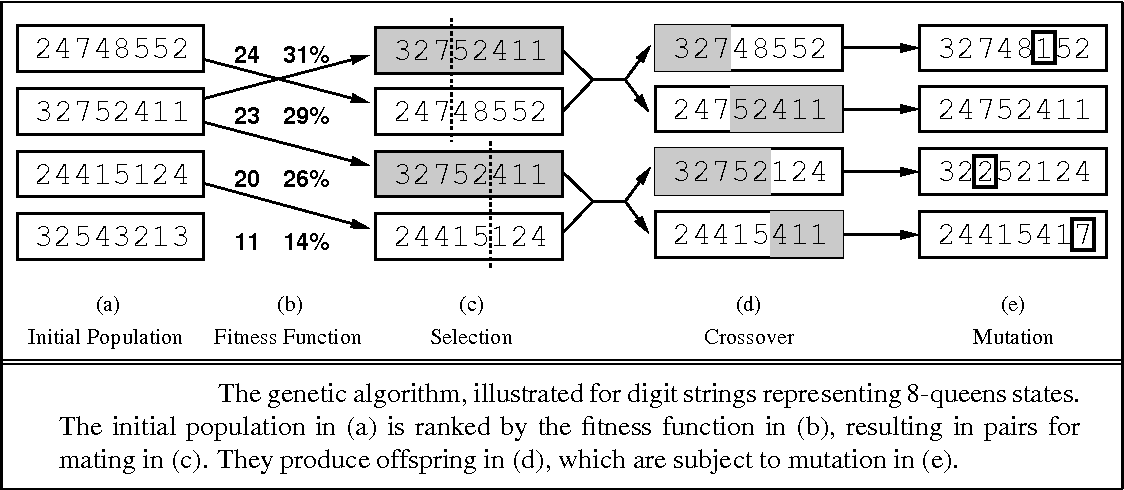
\includegraphics[width=0.85\textwidth]{0E4BagM.png}
	\end{figure}
\end{solution}
\noindent\rule{7in}{2.8pt}
\pagebreak
%%%%%%%%%%%%%%%%%%%%%%%%%%%%%%%%%%%%%%%%%%%%%%%%%%%%%%%%%%%%%%%%%%%%%%%%%
\end{document}
 